  %
%  $Description: Author guidelines and sample document in LaTeX 2.09$ 
%
%  $Author: ienne $
%  $Date: 1995/09/15 15:20:59 $
%  $Revision: 1.4 $
%

\documentclass[times, leqno,twocolumn]{article} 
\usepackage{icdm07}
\usepackage{times}
\usepackage{amsmath}
\usepackage{graphicx}

\newcommand{\THOR}{{{\tt THOR}} }

\newcommand{\authornote}[1]{\footnote{Note to self: #1}}
\newcommand{\authorsnote}[1]{\authornote{#1}}
\newcommand{\com}[1]{{\small \textit{((#1))}}}

\newcommand{\union}{\cup}
\newcommand{\intersect}{\cap}
\newcommand{\Union}{\bigcup}
\newcommand{\Intersect}{\bigcap}
\newcommand{\bigvec}[1]{\mathop{\overrightarrow{#1}}}

\newcommand{\otimeshat}{\widehat{\otimes}}
\newcommand{\odothat}{\widehat{\odot}}

\newcommand{\prefsplit}[2]{#1 \succ #2}
\newcommand{\summary}{\hat{\sigma}}

\DeclareMathOperator*{\map}{map}
\DeclareMathOperator*{\worst}{worst}
\DeclareMathOperator*{\argmin}{argmin}
\DeclareMathOperator*{\argmax}{argmax}
\DeclareMathOperator{\TWOPT}{TWOPOINT}
\DeclareMathOperator{\cardinality}{cardinality}
\DeclareMathOperator{\hrect}{hrect}
\DeclareMathOperator{\child}{child}
\DeclareMathOperator{\visited}{visited}
\DeclareMathOperator{\unvisited}{unvisited}
\DeclareMathOperator{\prune}{prune}
\DeclareMathOperator{\IF}{if}
\DeclareMathOperator{\ATDISCRETION}{}

\newcommand{\fig}[1]{Figure~\ref{fig:#1}}

\newcommand{\Gnp}{\Psi_{\Theta}}
\newcommand{\gnp}{\psi_{\Theta}}

%\newcommand{\psty}{\scriptstyle}
\newcommand{\psty}{}
\newcommand{\X}{\\ \psty}
\newcommand{\x}{\X \hspace{0.13in}}
\newcommand{\xx}{\X \hspace{0.26in}}
\newcommand{\xxx}{\X \hspace{0.39in}}
\newcommand{\xxxx}{\X \hspace{0.52in}}

\newcommand{\defterm}[1]{{\bf #1}}
\newcommand{\nbody}{$N$-body}

\newcommand{\kdroot}[1]{#1^{\text{root}}}
\newcommand{\kdleft}[1]{#1^{\!L}}
\newcommand{\kdright}[1]{#1^{\!R}}
\newcommand{\kdparent}[1]{#1^{\!P}}

\newcommand{\lo}[1]{#1^{l}}
\newcommand{\up}[1]{#1^{u}}
\newcommand{\distlo}{\lo{d}}
\newcommand{\distup}{\up{d}}
\newcommand{\dist}[2]{d(#1,#2)}

%\newcommand{\myOp}[1]{\mathop{\bigotimes\nolimits\hspace{-0.045in}_{#1}}}
\newcommand{\nameOp}[2]{\mathop{#1\nolimits\!\!_{#2}}}
\newcommand{\nameop}[2]{{\scriptstyle\:}#1_{\!#2}}
\newcommand{\myOp}[1]{\nameOp{\bigotimes}{#1}}
%\newcommand{\myop}[1]{\otimes\hspace{-0.04in}_{#1}\hspace{0.03in}}
\newcommand{\myop}[1]{\nameop{\otimes}{#1}}
\newcommand{\myOutop}[1]{\nameOp{\bigodot}{#1}}
\newcommand{\myoutop}[1]{\nameop{\odot}{#1}}

\newcommand{\letterglob}{\psi}
\newcommand{\outglob}{\Psi}
\newcommand{\inglob}{\psi}
\newcommand{\Opglob}{\myOp{\letterglob}}
\newcommand{\opglob}{\myop{\letterglob}}
\newcommand{\fglob}{f_{\!\letterglob}}
\newcommand{\gglob}{g_{\!\letterglob}}
\newcommand{\canpruneglob}{C_{\!\letterglob}}
\newcommand{\deltaglob}{\summary_{\!\letterglob}}

\newcommand{\letterqr}{\rho}
\newcommand{\outqr}{\varrho}
\newcommand{\inqr}{\rho}
\newcommand{\Opqr}{\myOp{\letterqr}}
\newcommand{\opqr}{\myop{\letterqr}}
\newcommand{\fqr}{f_{\!\letterqr}}
\newcommand{\gqr}{g_{\!\letterqr}}

\newcommand{\letterqrv}{\vec{\rho}}
%\newcommand{\outqrv}{\vec{\rho}}
\newcommand{\inqrv}{\vec{\rho}}
%\newcommand{\fqrv}{f_{\letterqrv}}
%\newcommand{\gqrv}{g_{\letterqrv}}
\newcommand{\deltaqrv}{\summary_{\!\letterqrv}}
\newcommand{\canpruneqrv}{C_{\!\letterqrv}}
\newcommand{\identqr}{0_{\!\letterqrv}}
\newcommand{\varqrv}{\letterqrv^{\:C\!}}
\newcommand{\varqrvparent}{\letterqrv^{\:P\!}}

\newcommand{\lettermu}{\mu}
%\newcommand{\inmu}{\mu}
\newcommand{\inmu}{\mu}
\newcommand{\Outopmu}{\widehat{\nameOp{\bigodot}{\lettermu}}}%\mathop{\widehat{\bigodot\nolimits}\!\scriptstyle{\mu}}}
\newcommand{\outopmu}{\:\widehat{\odot}_{\!\mu}\:}
\newcommand{\Opmu}{\myOp{\lettermu}}
\newcommand{\opmu}{\myop{\lettermu}}
\newcommand{\fmu}{f_{\!\lettermu}}
\newcommand{\fmuv}{\vec{f_{\!\lettermu}}}
\newcommand{\deltamu}{\summary_{\!\lettermu}}
\newcommand{\canprunemu}{C_{\!\lettermu}}
\newcommand{\heurqr}{H}
\newcommand{\identmu}{0_{\lettermu}}
\newcommand{\varmuchild}{\lettermu^{\!C}}
\newcommand{\varmuparent}{\lettermu^{\!P}}

%\newcommand{\muparent}{\inmu_{\text{coarse}}}
%\newcommand{\muchild}{\inmu_{\text{children}}}
%\newcommand{\muvisit}{\inmu_{\text{visited}}}
%\newcommand{\muall}{\inmu_{\text{all}}}

%\newcommand{\hatpi}{\hat{\outpi}}
%\newcommand{\piparent}{\outpi_{\text{parent}}}

\newcommand{\letterstat}{s}
\newcommand{\namestat}[1]{\sigma_{\text{#1}}}
\newcommand{\outstat}{\sigma}
\newcommand{\instat}{s}
\newcommand{\Opstat}{\myOp{\letterstat}}
\newcommand{\opstat}{\myop{\letterstat}}
\newcommand{\fstat}{f_{\!\letterstat}}
\newcommand{\gstat}{g_{\!\letterstat}}

% Affinity propagation


\newcommand{\eqspace}{\!\!\!\!}
\newcommand{\true}{\text{true}}
\newcommand{\ocpos}[1]{c^{+}_{#1}}
\newcommand{\ocneg}[1]{c^{-}_{#1}}
\newcommand{\cpos}[2]{\ocpos{#1 \neq #2}}
\newcommand{\cneg}[2]{\ocneg{#1 \neq #2}}

\newcommand{\respo}[2]{R_{#1#2}}
\newcommand{\avail}[2]{A_{#1#2}}
\newcommand{\simil}[2]{S_{#1#2}}

\newcommand{\vecrho}{\vec{\rho}}
\newcommand{\vecalpha}{\vec{\alpha}}
\newcommand{\frho}[1]{\rho_{#1}}
\newcommand{\falpha}[1]{\alpha_{#1}}
\newcommand{\falphaj}[2]{\alpha_{#1[#2]}}

\newcommand{\falphamax}{\alpha^{u}}
\newcommand{\falphamin}{\alpha^{l}}
\newcommand{\frhomax}{\rho^{u}}
\newcommand{\frhomin}{\rho^{l}}

\newcommand{\alphacand}{v}


%\documentstyle[times,art10,twocolumn,latex8]{article}

%------------------------------------------------------------------------- 
% take the % away on next line to produce the final camera-ready version 
\pagestyle{empty}

%------------------------------------------------------------------------- 
\begin{document}

%\title{Framework for Fast Parallel Generalized N-Body Methods}
\title{Parallelization of Generalized $N$-Body Methods}

\author{Garrett F. Boyer, Ryan N. Riegel, Alexander G. Gray
\\ Georgia Institute of Technology
\\ Computational Science and Engineering
\\ 801 Atlantic Drive, Atlanta, GA
\\ garryb@cc.gatech.edu
\\
% For a paper whose authors are all at the same institution, 
% omit the following lines up until the closing ``}''.
% Additional authors and addresses can be added with ``\and'', 
% just like the second author.
\and
\\ Robert Nichol
\\ University of Portsmouth
\\ bob.nichol@port.ac.uk
}

\maketitle
\thispagestyle{empty}

\begin{abstract}
The multi-tree approach for accelerating data mining methods has resulted some of the fastest known solutions for a large class of fundamental methods previously considered infeasible for massive datasets, including kernel density estimation, all-nearest-neighbor search, spatial statistics, and many others.
We present a standard mathematical model that allows these problems to be scaled further via parallelization, without significant extra programmer effort.
With the framework, we derive a strategy for parallelization and describe our implementation, Tree High-Order Reduce or \THOR.
We then demonstrate scalability for massive datasets in both multi-threaded and cluster settings.
\end{abstract}

\section{Introduction}

Many problems in spatial statistics and data mining, especially nonparametric methods, nominally require an all-pairs analysis of metric data.
Recent work\authorsnote{not yet officially published}\cite{ryan_nips} has characterized these {\it generalized $N$-body problems} and shown how a multi-tree algorithmic approach directly follows, leading quite often to asymptotically faster algorithms, sometimes nearly linear.
The multi-tree approach treats these problems by recursively dividing the problem over the Cartesian product of points along the axes of a space partitioning tree such as $kd$-tree, resulting in the fastest practical serial algorithms for many statistical and physical problems, such as kernel density estimation, $n$-point correlation, nearest neighbor finding, Gaussian process regression, and more.

Nonetheless, as multi-core processors begin to dominate even commodity markets, even the fastest serial algorithms may not compete with a trivially parallelizable brute-force algorithm.
Multi-tree algorithms traditionally excel in nonparametric learning, and since nonparametric perform exceptionally well with massive data, it is only natural to conceive of data mining the {\it entire Web} with efficient dual-tree algorithms.
Fortunately, multi-tree algorithms are in fact quite parallel, and we show how the techniques that have long been used to parallelize the physical $N$-body force calculation problems can be extended to encompass this broader class of problems.

\section{Fast Dual-Tree Algorithms}

\begin{figure*}
  \begin{minipage}{6in}
    \begin{minipage}{2.5in}
      \begin{displaymath}
        \begin{array}[t]{l}
          \text{{\bf tpc} - Two-point correlation.}
          \X \text{function tpc}(Y, X)
          \x \text{if }\distup(Y, X) > h\text{, return }0
          \x \text{if }\distlo(Y, X) \leq h\text{, return } |Y| \cdot |X|
          \x \text{else if }|Y| \geq |X|\text{,}
          \xx \text{return tpc}(\kdleft{Y}, X, h) + \text{tpc}(\kdright{Y}, X, h)
          \x \text{else,}
          \xx \text{return tpc}(Y, \kdleft{X}, h) + \text{tpc}(Y, \kdright{X}, h)
        \end{array}
       \end{displaymath}
       \caption{\footnotesize \label{fig:allnntpc} Pseudocode for two simple dual-tree algorithms.}
      \end{minipage}
      \begin{minipage}{3.0in}
       \begin{displaymath}
        \begin{array}[t]{l}
          \text{{\bf allnn} - All-nearest-neighbors.}
          \X \text{init all nodes }Q \subseteq \kdroot{Q}\text{, }a(Q) \gets \infty
          \X \text{procedure allnn}(Q,R)\text{,}
          \x \text{if }a(Q) < \distlo(Q, R)\text{, return}
          \x \text{else if }Q = \{q\} \text{ and } R = \{r\}
          \xx a(\{q\}) \gets \min(a(\{q\}), \dist{Q}{R})
          \x \text{else if }|Q| \geq |R|\text{,}
          \xx \text{allnn}(\kdleft{Q}, R); \text{ allnn}(\kdright{Q}, R)
          \xx a(Q) \gets \max(a(\kdleft{Q}), a(\kdright{Q}))
          \x \text{else prioritize by min distance,}
          \xx \text{allnn}(Q, \kdleft{R}); \text{ allnn}(Q, \kdright{R})
        \end{array}
       \end{displaymath}
      \end{minipage}
  \end{minipage}
\end{figure*}

\authornote{KD-tree figure goes here}
Spatial trees and bounds form the core of tree algorithms.
Every node $X$ in a spatial tree $\kdroot{X}$ is a set of points; every internal node is partitioned $\kdleft{X} \union \kdright{X} = X$ with parent $\kdparent{X}$, with each leaf a single point $\{x\}$\footnote{In practice, leaves contain multiple points to amortize recursion overhead.}.
For example, a $kd$-tree\cite{preparata_kdtrees}, as in \fig{kdtree}, recursively partitions the data along coordinate dimensions.
Each node has a bounding box and can also store summary statistics such as means and other moments.
Notationally, we denote $\dist{x}{y}$ to be a distance metric such as Euclidean $||x-y||$.
Superscripts $l$ and $u$ refer respectively to lower and upper bounds, which are often, as in the case of distance, obtained from the node's bounding box.

\authornote{This paragraph needs some work.}A single-tree algorithm accelerates computation by partitioning reference data, such as training data, in half along the tree branches.
When considering a query point, such as a test datum, some parts of the tree bear no computational relevance or can be summarized at a coarse level, and the subcomputation is pruned.
Since this traversal is frequently repeated for many query points, a dual-tree algorithm further accelerates by building a tree over queries.
It is then possible to look at {\it pairs} of nodes, each time partitioning the Cartesian product of queries and references in half.
Whereas a single-tree algorithm must consider every level of the tree for each query point and is at best $O(N \log N)$, a dual-tree algorithm considers the upper-level nodes of the tree only with other upper-level nodes, leading at times to linear performance.
The dual-tree approach, despite its simplicity, leads to a multitude of asmyptotically fast algorithms.

{\bf The Two-point Correlation.}
A member of the family of $n$-point correlation functions, collectively the foundation for all spatial statistics, the two-point correlation of a data set is the number of pairs of points within a specified radius.
For data set $X$, radius $h$, and indicator function $I$, it can be expressed
$\sum_{x \in X} \sum_{y \in X} I(d(x, y) \leq h)$.
Figure~\ref{fig:allnntpc} shows a formulation that recursively considers a subset pair $Y$ and $X$, returning immediately if all points in $Y$ and $X$ are completely inside or outside the radius.
The asmyptotic speedul of this dual-tree algorithm was shown in \cite{gray_nips}.

{\bf All-nearest-neighbors.}
In applications from manifold learning to classification, one computes the nearest neighbors from reference set $R$ for a batch of queries $Q$.
We express this computation $\map_{q \in Q} \argmin_{r \in R} d(q,r)$.
To achieve speedup, one maintains for each tree node $Q$ of queries the furthest candidate neighbor distance, $a(Q)$.
If a set of references is farther away than this distance, no further exploration is required.\authorsnote{Publish this algorithm}

{\bf Kernel density estimation.}
By placing a kernel such as a multivariate Gaussian or Epanechnikov kernel at each data point, it is possible to estimate the overall probability density of a multi-dimensional data set.
Given a kernel $K$, data set $R$, and query points $Q$, calculate $\map_{q \in Q} \sum_{r \in R} K(q, r)$.
A dual-tree algorithm \cite{gray_kde, dong_kde} can be used to give a bounded relative-error approximations for each query point, by pruning subcomputations with acceptable error.

{\bf Affinity propagation.}
Affinity propagation is a recent clustering technique that identifies exemplars in a data set, taking into account all point-to-point similarities\cite{affinity}\authorsnote{I might not actually implement this in parallel}.
The similaritiy $\simil{i}{j}$ between points $x_i$ and $x_j$ is the negative squared distance or some other quantity to be maximized, with diagonals $\simil{i}{i}$ set to a parameter that controls the number of clusters.
The algorithm maximizes the sum of similarities between each point and its chosen exemplar.
If a metric space is defined over the points, one use the dual-tree algorithm in \cite{ryan_nips} to solve a modified version of the affinity propagation update steps,
\[ \begin{array}{l}
  \vecalpha \gets \map_{i} \argmin^2_{j} \!\left( \cpos{i}{j}(\cpos{i}{j}(\simil{i}{j} + \falphaj{i}{j}) - \frho{j}) - \simil{i}{j} \right)\! ,
  \\
  \vecrho \gets \map_{j} \sum_{i} \!\left( \cpos{i}{j}(\simil{i}{j} + \falphaj{i}{j}) \right)\!,
\end{array} \]
\noindent with $\ocpos{v}(x)$ being $\min(x, 0)$ for $v$ true and $x$ otherwise, and $\falphaj{i}{j}$ being the first minimum of $\falpha{i}$ when $i \neq j$ and the second otherwise.
%These vectors are computed iteratively until convergence.
%Exemplars are those points $j$ with $\frho{j}$ positive and each point belongs to the cluster defined by the exemplar closest to it.
The algorithm uses $O(N)$ space and empirically took $O(N^{1.3})$ on three-dimensional points from a gravitational $N$-body particle simulation, compared to the existing $O(N^2)$ time and space method.

{\bf Generalization.}
All of these problems have a characteristic of nested commutative, associative operators over an inner computation.
Indeed, we later show this property is essential to both dual-tree algorithms and their parallelization.

\section{Parallel $N$-Body Simulations}

$N$-body particle simulations comprise some of the best-studied parallel computing problems.
Algorithms for efficient simulation almost universally use trees, and parallelization of these tree codes offers indispensible insight into that of generalized $N$-body problems.
The physical $N$-body problem models $N$ particles in an evolving system where each particle exerts force on all other particles.
Computational solutions break the simulation into discrete time steps, during which force is calculated,
\[\map_{q \in D} \sum_{r \in D} f(q,r)\]
\noindent where $f(q,r)$ is often an inverse-squared-distance gravitational or Coulombic force.
Directly computing the sum takes $O(N^2)$ time, but speedup is achieved by approximating distant interactions.

The popular Barnes-Hut algorithm\cite{barnes_hut} and Fast Multipole Method\cite{greengard_fmm} received significant attention from the parallelization community.
Barnes-Hut\cite{barnes_hut} descends an oct-tree\footnote{An oct-tree hierarchically divides all 3 dimensions at the midpoint.} to approximate force on each particle.
If query particle $q$ is further than parameter $\theta$ times the spatial width of the considered node, the force calculation is approximated by the node's center of mass.
Although Barnes-Hut is a single-tree algorithm, many aspects of its parallelization can often be generalized to the dual-tree case.

The Fast Multipole Method (FMM)\cite{greengard_fmm} achieves closer to $O(N)$, but with a higher constant factor than the $O(N log N)$ Barnes-Hut, by considering node-node interactions like dual-tree algorithms.
Although the FMM may be posed as a dual-tree algorithm due to its node-node computations, it has a very specific descent pattern.
Thus, the details of a parallel implementation of the FMM cannot be entirely transferred to dual-tree algorithms, although some features in common.

% \cite{singh95load} \cite{nyland93dataparallel} \cite{washington_nesl}

\section{Parallel Programmability}

Making parallelization accessible to algorithm developers without parallelization expertise has been a common goal in parallelization communities.
In this realm, there are three general approaches.

At the highest level, the programming languages community attempts either to create languages that are functional and inherently parallel or to add parallel extensions to existing programming languages.
For instance, the Barnes-Hut and the Fast Multipole Method have both been parallelized with the NESL parallel programming language, and \cite{hu-implementing, more}\authorsnote{I need to read their papers}.
Languages like UPC attempt to make parallelizable C code, but only for algorithms with stereotypically "linear" access patterns or data decompositions.
Unfortunately, these are typically so high-level that it is not possible to control what underlying techniques are used.
Although not completely unpredictable, the access pattern of an $N$-body problem is far from static, and trivial work decompositions are impractical.

Alternately, at the lowest level, projects like SAM\cite{sam} provide a distributed memory layer that abstracts physically distributed memory as one logical address space, except that it provides versioned values or accumulators instead of implementing a coherency model.
The authors of SAM achieved over 50\% speedup for about 64 processors for the Barnes-Hut algorithm on various parallel computers.
Another low-level abstraction simply simulates distributed RAM using a lazy consistency protocol by listening for segmentation faults\cite{relaxed}.
They also implemented, as an example, a version of Barnes-Hut that scaled to about 8 processors.

Another popular approach requires identifying a specific, but diverse, class of problems that share common properties.
It may be possible to create a very efficient implementation with arbitrarily complex low level details for the entire problem class, allowing the developer to plug in the specifics of their problem.
One popular example is Map-Reduce, a framework to solve problems that process massive data sets through the three-step process of preprocessing, sorting, and reduction.
By targetting this class of problems, Map-Reduce can use optimally efficient data decomposition methods, out-of-core sorting algorithms, and mechanisms for fault-tolerance.
Additionally, very little work on the part of the programmer is needed, so that sometimes writing the parallel algorithm can be simpler than writing the serial algorithm.

Due to the generalizability of $N$-body methods, \THOR takes the same approach as Map-Reduce to implement a highly specialized parallel version of the serial algorithm.
The developer needs only to focus on the interactions that occur among points and nodes, not on the details of the tree algorithm or its parallelization.
Additionally, since programmers prefer to use common constructs such as vectors and lists over static bit-copiable structures, \THOR provides a scheme that takes advantage of C++ templates to implement serialization and deserialization of acyclic pointer graphs, using a templated object traversal.
Thus, we present \THOR as a ``quick and easy'' way to generate parallel dual-tree algorithms that are also efficient.

\section{Dual-Tree Algorithm Framework}

\cite{ryan_nips} formalizes the class of generalized $N$-body problems and shows how they lead naturally to dual-tree algorithms.
We mention key points in order to motivate a unified computational model for generalized $N$-body problems.

A \defterm{second-order reduce problem} is a tuple $\Theta = (\mathcal{X}, \mathcal{Y}, \bigotimes, \bigodot, f, g, h)$ with $\bigotimes$ and $\bigodot$ both commutative and associative, such that for problem instance $X \subset {\mathcal{X}}, Y \subset {\mathcal{Y}}$, one computes
\[\begin{array}{l}
  \displaystyle \Gnp(X, Y) = h(\gnp(X, Y)),
  \\
  \displaystyle \gnp(X, Y) = \bigodot_{x \in X} g\!\left(x, \bigotimes_{y \in Y} f(x, y) \right).
\end{array}\]
\noindent For example, three-dimensional two-point correlation with radius $h$ is has,

\[\begin{array}{rcl}
  \mathcal{X} \equiv \mathcal{Y} &\equiv& \mathcal{R}^3
  \\
  \bigodot \equiv \bigotimes &\equiv& \sum
  \\
  f(x,y) &\equiv& I(d(x,y) < h)
  \\
  g(x, a) &\equiv& a
  \\
  h(b) &\equiv& b
\end{array}{c}\]
\noindent \authorsnote{use mathbb for reals}
A second-order reduce problem is \defterm{block decomposable} if for any partitioning $\kdleft{Y} \union \kdright{Y} = Y$, $\gnp(X,Y) = \gnp(X,\kdleft{Y}) \otimes \gnp(X,\kdright{Y})$.
We define a \defterm{generalized $N$-body problem} to be any block decomposable second-order reduce problem.

Two major types of regular reduce problems are block decomposable.
If $\bigodot = \bigotimes$ then associativity trivially leads to block decomposability; we call this a \defterm{single-operator second-order reduce problem}.
If $\bigodot$ is the special higher-order operator $\map$, then the problem can be formally expressed as block-decomposable by viewing it as a key-value pair problem, although such formality is not necessary in our discussions.
We term a $\map$ problem as \defterm{query-reference problem} since each result is specific to a particular query.

We finally note that {\it any} second-order reduce problem can be transformed into a query-reference GNP by replacing the outer operator with $\map$, treating both $g$ and $\odot$ as a postprocessing step.
Therefore, any parallelization framework that solves query-reference problems necessarily solves any second-order reduce problem.
Although \THOR has native support for both single-operator and query-reference problems, our discussion focuses on the more general query-reference problem.

{\bf The Generalized $N$-Body Algorithm.}
Block decomposition implies a hierarchical computation,
\[
\gnp(X,Y) = \left\{ \begin{array}{lrr}
    f(x,y) & \multicolumn{2}{r}{\text{if }X = \{x\}\text{ and }Y = \{y\}\text{,}}
    \\
    \multicolumn{2}{l}{\gnp(\kdleft{X},Y) \otimes \gnp(\kdright{X}, Y)} & \text{if }\prefsplit{X}{Y}\text{,}
    \\
    \multicolumn{2}{l}{\gnp(X,\kdleft{Y}) \odot \gnp(X,\kdright{Y})} & \text{otherwise,}
  \end{array}
\right.
\]
\noindent where $\prefsplit{X}{Y}$ specifies a recursion preference.
This hierarchical computation motivates the popular use of trees in generalized $N$-body problems.
A single-tree execution has $\prefsplit{X}{Y} = |X| > 1$, that is, $X$ is split until individual points are considered, after which $Y$ is recursed.
A dual-tree execution may use a heuristic such as $|X| \geq |Y|$ to prefer working on node pairs with approximately equal cardinality.
The \defterm{generalized $N$-body algorithm} initially considers the expression $\gnp(\kdroot{X}, \kdroot{Y})$, continually replacing any subexpression $\gnp(X, Y)$ with its expansion as mentioned above.
The final expression forms an \defterm{expression tree} where leaves are of the form $f(x,y)$ and internal nodes are either $\odot$ or $\otimes$.

For efficient computation, each node in the data tree has a statistic $\outstat(X)$ that may contain arbitrary problem-specific information, such as bounding box, mean, or variance.
Using these statistics, GNP's often can efficiently bound the results for $\gnp(X,Y)$ using a conceptual set \defterm{initial summary results} $\summary(\outstat_X,\outstat_Y) \supseteq \{\gnp(X',Y') | \outstat(X')\!\!=\!\!\outstat_X, \outstat(Y')\!\!=\!\!\outstat_Y\}$, that is, all results possible given a pair of statistics.
If this set is singleton, only one result is possible, and an \defterm{intrinsic prune} may be performed; this result becomes a leaf in the expression tree.

Sometimes the summary results of the entire problem imply that a subproblem needs no further consideration.
Summary results can be aggregated bottom-up in the same manner the problem has been decomposed using some summary composition operator $A \otimeshat B \supseteq \{a \otimes b | a \in A, b \in B\}$ and likewise for $\odothat$.
Unfortunately, these formal sets are infeasible to construct in practice, but can be bounded by considering single values that a represent a bound for a relevant part of the computation.
An example is the upper bound nearest neighbor distance kept by nearest neighbors for each query node.
%For all-nearest-neighbors, this set is the set of all sets of possible key-value pairs representing query points and the corresponding possible nearest neighbor distances, each of which ranges continuously from 0 (the best distance possible) to the best candidate nearest neighbor distance.
%A prune is made by intersecting this with the similar set returned by $\summary(\outstat(X),\outstat(Y))$, and if the summary result set is unaffected, $(X,Y)$ may be skipped entirely.
%Unfortunately, it is infeasible to represent this construct directly in practice, so typically a single upper and/or lower bound is stored to summarize worst-case bounds.

%The generalized $N$-body algorithm begins with $\gnp(\kdroot{X},\kdroot{Y})$, and repeatedly replacing some $\gnp(X,Y)$ with one of its expansions.
%There is no one required exploration pattern.
It is worth noting that the generalized algorithm is agnostic to expansion pattern, but individual algorithms may exhibit differing runtime performances.
If there is no extrinsic pruning rule, then $\prefsplit{X}{Y}$ solely determines the pruning behavior, with any expansion pattern behaving similarly.
Some problems that use extrinsic pruning may prefer a depth-first expansion if relevant data are almost always local, providing only a heuristic on which node pairs to expand first.
Others achieve good performance by a breadth-first expansion, that is similar to an "iterative refinement" of the computation.
Further expansion patterns may involve parallelism, by noting that, with a few performance implications, each subproblem can be considered independent.

%Ongoing research attempts to characterize all generalized N-body problems with rigorous mathematical formality; however, such rigorous formalization is outside the scope of this paper.
%Here, we postulate that all dual-tree algorithms fall into one or both of two categories: a single scalar or vector result summarizing all pairs of inputs, or an independent result for each query point computed against the entire reference set.

%A global reduction computes a single scalar or a vector of results that is constant with the number of data points.
%This type of problem is typically characterized by a single commutative, associative operator applied to pairs of inputs.
%Such problems include 2-point correlation, kernel-based data likelihood estimates, and the closest-pair problem.

%A query-reference problem alternatively computes a result for each point in a query set.
%For each point in the query set, execute a commutative, associative operator over every element in a reference set.
%These problems include such fundamental problems as all-nearest-neighbors, kernel density estimation, the testing phase of most nonparametric classification methods, matrix-vector multiplication, and many more.

%\subsection{Single-Operator Reduce Problems}
%
%A \defterm{single-operator reduce problem} computes a single scalar or relatively small vector of results, taking as input two data sets and applying an aggregate commutative and associative operator to all pairs,
%\begin{eqnarray*}
%\outglob(X, Y) &=& \gglob(\inglob(X, Y)),
%\\
%\inglob(X, Y) &=& \Opglob_{(x, y) \in X \times Y} \fglob(x, y).
%\label{eqn:defglob}
%\end{eqnarray*}
%
%\noindent where $\gglob$ is a post-processing function (usually identity), $\Opglob$ is a commutative and associative operator, and $\fglob$ is an inner function.
%We can express two-point correlation,
%\[\begin{array}{rcl}
%\TWOPT(X, r) &\equiv& \inglob_r(X, X),
%\\
%\opglob &\equiv& +
%\\
%\fglob(x, y) &\equiv& I(d(x, y) < h).
%\end{array}\]
%
%\noindent We decompose $\inglob$ with the identities,
%\begin{eqnarray*}
%\inglob(X, Y) &=& \inglob(\kdleft{X}, Y) \opglob \inglob(\kdright{X}, Y),
%\\
%\inglob(X, Y) &=& \inglob(X, \kdleft{Y}) \opglob \inglob(X, \kdright{Y}).
%\label{eqn:divideglob}
%\end{eqnarray*}
%
%\noindent and can be computed bottom-up $\instat(X) = \instat(\kdleft{X}) \opstat \instat(\kdright{X})$.
%Intrinsic prunes are applied with the following rule,
%\begin{equation*}
%\text{if } \canpruneglob(\outstat(X), \outstat(Y)) \text{, then } \inglob(X, Y) = \deltaglob(\outstat(X), \outstat(Y))
%\label{eqn:intrinsic}
%\end{equation*}
%\noindent where $\canpruneglob$ is a Boolean indicator that a prune is possible i.e. the initial summary set is singleton, and $\deltaglob$ is the summary set's only element.
%
%The rules shown so far allow some software system to execute single-operator reduce problems with intrinsic prunes given definitions for the relevant functions and operators.
%For instance, a $kd$-tree-based two-point correlation $\TWOPT(X, h)= \outglob(X,X)$ is defined:
%\begin{eqnarray*}
%\label{eqn:tpc_gglob}
%\gglob(\inglob) &\equiv& \inglob
%\\
%\label{eqn:tpc_opglob}
%\opglob &\equiv& +
%\\
%\label{eqn:tpc_fglob}
%\fglob(x,y) &\equiv& I(\dist{x}{y} < h)
%\\
%\label{eqn:tpc_canpruneglob}
%\canpruneglob(\sigma(X), \sigma(Y))
%&\equiv&
%\begin{array}{l}\distup(\outstat(X),\outstat(Y)) < h \\ \vee \distlo(\outstat(X),\outstat(Y)) \geq h\end{array}
%\\
%\label{eqn:tpc_deltaglob}
%\deltaglob(\outstat(X),\outstat(Y)) &\equiv& \left\{ \begin{array}{l} 0 \text{ if } \distup(\outstat(X),\outstat(Y)) < h \\ |X|\cdot|Y| \text{ if } \distlo(\outstat(X),\outstat(Y)) \geq h \end{array}\right.
%\\
%\label{eqn:tpc_fstat}
%\fstat(x) &\equiv& (x,x)
%\\
%\label{eqn:tpc_opstat}
%\opstat(x) &\equiv& \left( \bigvec{\min} , \bigvec{\max} \right)
%\end{eqnarray*}
%\noindent The first three summarize the problem itself, with the next two specifying the pruning condition.
%The last two specify the construction of a bounding box, although this is automatic with $kd$-trees.
%Given a parallel execution system, the above is all the programmer needs to specify to have a fully parallelized two-point correlation.
%

%The model shown so far is limited to very simple dual-tree algorithms.
%First, we later discuss additions to allow for efficient computation of query-reference problems such as all-nearest-neighbors and density estimation.
%Additionally, many algorithms, such as nearest-neighbor, classification problems, and approximate density estimates, require information about previous pairwise computation in order to determine whether pruning is possible.
%Nonetheless, this simple model leads to effective parallelization of problems such as two-point correlation\footnote{list more}.

\subsection{Simple Query-Reference Problems}
A query-reference problem computes for each query $q$,
\begin{eqnarray*}
\outqr(q, R) &=& \gqr(q, \inqr(q, R)),
\\
\inqr(q, R) &=& \Opqr_{r \in R} \fqr(q, r).
\end{eqnarray*}

\noindent where $R$ is initially $\kdroot{R}$.
In addition to the classic \nbody\ force calculation problem, this encompasses all-nearest-neighbors, k-nearest-neighbors classification, kernel density estimation, affinity propagation, and more.
 Although each query is independent, speedup is achievable by considering queries {\it en masse}; that is, the contribution of a set of references might be shown to have an exact value for an entire distant set of queries.
A \defterm{mass result} $\inqrv(Q, R)$ is defined if it is acceptable to treat
\[
\forall q \in Q,~~ \inqr(q, R) \gets \inqrv(Q, R)
\]
\noindent within the context of the entire computation.
Otherwise, $\inqrv(Q,R)$ is undefined.
%different queries have different values after the postprocessing function is applied, although for a single query $\inqrv(\{q\}, R)$ can always be computed $\inqr(q, R)$.
In a dual-tree algorithm, we may take advantage of $\inqrv$,
\begin{equation*}
\text{if prune occurs for } \kdparent{Q} \supset Q \text{, then } \inqrv(Q, R) = \inqrv(\kdparent{Q}, R).
\label{eqn:parentqrv}
\end{equation*}

\noindent
A single-tree algorithm treats each query as a separate computation and does not distinguish $\inqrv$ and $\inqr$.
Both algorithms, though, compute values by dividing along the reference tree,
\begin{equation*}
\inqrv(Q, R) = \inqrv(Q, \kdleft{R}) \opqr \inqrv(Q, \kdright{R}),
\label{eqn:dividepi}
\end{equation*}
\noindent perhaps with an intrinsic prune,
\begin{equation*}
\text{if } \canpruneqrv(\outstat(Q), \outstat(R)) \text{, then } \inqrv(Q, R) = \deltaqrv(\outstat(Q), \outstat(R)).
\label{eqn:prunepi}
\end{equation*}

\noindent
where the statistics $\outstat(Q)$ and $\outstat(R)$ are commonly built from commutative associative operators, and may also be decomposed:

\begin{eqnarray*}
\outstat(X) &=& \gstat(\instat(X)),
\\
\instat(X) &=& \Opstat_{x \in X} \fstat(x),
\label{eqn:defstat}
\end{eqnarray*}

\noindent Range count, the query-reference analog to two-point correlation $\map_{q \in Q} \sum_{r \in R} I(\dist{q}{r} < h)$ is\footnote{When I use deltas, make sure I consistently put the sigmas as the arguments.}:
\begin{eqnarray*}
\gqr(q, \inqr) &\equiv& \inqr
\\
\opqr &\equiv& +
\\
\fqr(q,r) &\equiv& I(\dist{q}{r} < h)
\\
\canpruneqrv(\sigma(Q), \sigma(R))
&\equiv&
\begin{array}{l}\distup(\outstat(Q),\outstat(R)) < h \\ \vee \distlo(\outstat(Q),\outstat(R)) \geq h\end{array}
\\
\deltaqrv(\outstat(Q),\outstat(R)) &\equiv& \left\{ \begin{array}{l} 0 \text{ if } \distup(\outstat(Q),\outstat(R)) < h \\ |R| \text{ if } \distlo(\outstat(Q),\outstat(R)) \geq h \end{array}\right.
\end{eqnarray*}

\noindent
The two-point correlation may be computed by summing $\outqr$ for all queries.

\subsection{Query-Reference Extrinsic Prunes}

Extrinsic pruning in a query-reference problems is a more complex process but still leads to an overarching model\footnote{Single-operator reduce problems have this kind of prune too, but since it is less common, we have omitted it for brevity.}.
We define the abstract $\inmu(Q, R)$ as a compact representation of the summary results for the computation $(Q,R)$.
At completion, we desire the ideal value $\inmu(Q, \kdroot{R})$ for each query node with
\begin{equation*}
\inmu(Q, R) \gets \Outopmu_{q \in Q} \fmu(q, \inqr(q, R)).
\end{equation*}

\noindent where $\Outopmu$ is a commutative and associative operator that merges representative summary results among queries, such as finding the worst candidate nearest neighbor distance in all-nearest-neighbors.
Although the generalized $N$-body algorithm states that summary results are built in the same structure as the refinement pattern, practical considerations encourage storing at each query node the best possible bounds for that node; for this reason, we start with this rather contrived definition.
We can merge two subcomponents trivially\authorsnote{Emphasize that we're not necessarily talking about tree structures, just disjoint parts of the tree.},
\begin{equation*}
\inmu(Q, R) \gets \inmu(\kdleft{Q}, R) \outopmu \inmu(\kdright{Q}, R).
\label{eqn:dividemu}
\end{equation*}

\noindent The value of $\inmu(Q, \kdroot{R})$ is used to make pruning decisions via the modified $\canprunemu(\outstat(Q), \outstat(R), \inmu(Q, \kdroot{R}))$.
During computation, it is more realistic to compute $\inmu$ from statistics, or from other estimations of $\inmu$.
One may bound $\inmu$ using summary statistics,
\begin{equation*}
\inmu(Q, R) \gets \deltamu(\outstat(Q), \outstat(R)).
\label{eqn:approxmu}
\end{equation*}

\noindent Next, if we know $\inmu$ for two different references, we may compose them in a way analagous to the original $\Opqr$,
\begin{equation*}
\inmu(Q, R) \gets \inmu(Q, \kdleft{R}) \opmu \inmu(Q, \kdright{R}).
\label{eqn:combinemu}
\end{equation*}

\noindent It is important to note that the above may be quite pessimistic.
Since it treats all the queries in the node as one, it cannot for instance realize that the ``worst'' result for one set of references occurs at a particular query point, whereas the ``best'' result occurs at the same query point for another set of references.
%For example, if $\inmu$ is an upper bound on a probability density contribution, summing the upper bounds neglects the possibility of having the upper bound appear at different query points for the two subcomputations.
%\authornote{Elaborate more, or make less comments.  Actually, this might want a proof.}
Next, if $\inqrv(Q, R)$ is defined because this computation was pruned, then we may bound its worst-case contribution until the value of $\inqrv$ is propagated to $\inqr$ for all points in $Q$,
\begin{equation*}
\inmu(Q, R) \gets \fmuv(\outstat(Q), \inqrv(Q, R)).
\label{eqn:pimu}
\end{equation*}

\noindent 
Finally, the summary information for any set of queries must necessary reflect all contained queries, and thus be valid for all its children.
When no other information is available, we must resort to this rule, especially when performing depth-first expansions,
\begin{equation*}
\inmu(Q, R) \gets \inmu(\kdparent{Q}, R) \text{ if } \kdparent{Q} \supset Q.
\end{equation*}

\noindent {\bf Quality.} A final note is that extrinsic pruning requires ``high-quality'' values of $\inmu$, that is, values that approach the aforementioned ideal value.
The quality of $\inmu$ generally increases as more node pairs are explored\authorsnote{In reality, exploring a node pair should never decrease the quality, although uninformed implementations that use ball-trees might exhibit this condition.}, but the exploration pattern is extremely important.
The distribution over node pairs of information yield potential is highly non-uniform in efficient dual-tree problems, and thus prioritization is used to focus on node pairs with higher potential information yield.
A heuristic function $\heurqr(\outstat(Q),\outstat(R))$ returns a real value where lower values are explored first.
Finding all nearest neighbor distances then becomes,
\begin{eqnarray*}
\gqr(q, \inqr) &\equiv& \inqr
\\
\opqr &\equiv& \min
\\
\fqr(q,r) &\equiv& \dist{q}{r}
\\
\heurqr(\outstat(Q),\outstat(R)) &\equiv& \distlo(\outstat(Q), \outstat(R))
\\
\canprunemu(\sigma(Q), \sigma(R), \lettermu)
&\equiv&
\lettermu < \distlo(\outstat(Q), \outstat(R))
\\
\deltaqrv(\outstat(Q),\outstat(R)) &\equiv& \infty
\\
\outopmu &\equiv& \max
\\
\opmu &\equiv& \min
\\
\fmu(q, \letterqr) &\equiv& \letterqr
\\
\fmuv(\outstat(Q), \letterqrv) &\equiv& \letterqrv
\\
\deltamu(\outstat(Q),\outstat(R)) &\equiv& \distlo(\outstat(Q),\outstat(R))
\end{eqnarray*}

\noindent One small note is that in depth-first implementations, $\deltamu$ is typically ignored, i.e. treated as $\infty$, such that unvisited references are ignored.
However, in breadth-first and other patterns, $\deltamu$ is essential\authorsnote{Does $\deltaqrv$ want to take in $\lettermu$ as a parameter?}.

\subsection{Examples}

Note to self: I could put an examples section, and talk about how we handle things like the fast multipole method (which is really the distributive property of $\fqr$ with $\opqr$).

\subsection{Execution}

We show in \fig{dfe} a depth-first implementation of the query-reference with extrinsic prune rules for query-reference problems\footnote{The code for single-operator problems is much simpler, and \THOR actually can compute both simultaneously.}
The input to the algorithm consists of the data to operate on and the functions required for an effective dual-tree algorithm.
Via the power of $\map$, we have shown that this code can solve any second-order reduce problem.
\THOR also has a breadth-first implementation that performs far better for some problems.

\begin{figure}
\[
  \begin{array}[t]{l}
    \\ \text{Input:}\left(
        \begin{array}[c]{l}\kdroot{Q}, \kdroot{R}, \gqr, \opqr, \fqr, \deltaqrv, \\ \heurqr, \canprunemu, \outopmu, \opmu, \fmuv, \deltamu\end{array}\right)
    \X \text{for all nodes } Q \in \kdroot{Q}\text{: } \varmuchild(Q) \gets \text{identity of }\Opmu
    \X \text{for all nodes } Q \in \kdroot{Q}\text{: } \varqrv(Q) \gets \text{identity of }\Opqr%\identqr
    \X \text{dfe}(\kdroot{Q}, \kdroot{R}, \text{identity of }\Opmu)
    \X \text{fixup}(\kdroot{Q}, \identqr)
    \X
    \X \text{procedure dfe}(Q, R, \varmuparent)\text{:}
    \x \!\!\!\begin{array}{lllll}
         \psty\inmu(Q,\kdroot{R}) &\psty\!\!\gets\!\!& \psty\varmuchild(Q) &\psty\!\!\opmu\!\!& \psty\fmuv(\outstat(Q), \varqrv(Q))
         \\              &\psty\!\!\opmu\!\!& \psty\varmuparent   &\psty\!\!\opmu\!\!& \psty\deltamu(\outstat(Q), \outstat(R))
       \end{array}
    \x \text{if } \exists q \exists r ~ Q = \{q\} \wedge R = \{r\}\text{: \com{base case}}
    \xx \varqrv(\{q\}) \gets \varqrv(\{Q\}) \opqr \fqr(q, r)
    \x \text{else if } \canprunemu(\outstat(Q), \outstat(R), \inmu(Q,\kdroot{R}))\text{: \com{prune}}
    \xx \varqrv(Q) \gets \varqrv(Q) \opqr \deltaqrv(\outstat(Q), \outstat(R))
    \x \text{else if } |Q| \geq |R|\text{: \com{explore queries}}
    \xx \text{for } Q' \in \{\kdleft{Q}, \kdright{Q}\}\text{:}
    \xxx \varqrv(Q') \gets \varqrv(Q') \opqr \varqrv(Q)
    \xxx \text{dfe}(Q', R, \varmuparent)
    %\xx \text{let }\muvisit(Q') \gets \muchild(Q') \opmu \gpiworst(\outstat(Q'), \hatpi(Q'))
    \xx \varqrv(Q) \gets \text{identity of }\Opqr
    \xx \!\!\!\begin{array}{lll}
         \psty \varmuchild(Q) &\psty\!\!\gets\!\!&\psty (\varmuchild(\kdleft{Q})  \opmu \fmuv(\kdleft{Q}, \varqrv(\kdleft{Q})))
         \\          &\psty\!\!\outopmu\!\!&\psty (\varmuchild(\kdright{Q}) \opmu \fmuv(\kdright{Q}, \varqrv(\kdright{Q})))
        \end{array}
    \x \text{else: \com{explore references}}
    \xx (R_a, R_b) \gets \text{sort }(\kdleft{R}, \kdright{R})\text{ by }\lambda v ~ \heurqr(\sigma(Q), \sigma(v))
    \xx \text{dfe}(Q, R_a, \varmuparent \opmu \deltamu(\outstat(Q), \outstat(R_b))
    \xx \text{dfe}(Q, R_b, \varmuparent)
    \X
    \X \text{function fixup}(Q, \varqrvparent)\text{:}
    \x \varqrv(Q) \gets \varqrv(Q) \opqr \varqrvparent
    \x \text{if } \exists q ~ Q = \{q\}\text{:}
    \xx \outqr(q, \kdroot{R}) \gets \gqr(q, \varqrv(Q))
    \x \text{else:}
    \xx \text{fixup}(\kdleft{Q}, \varqrv(Q))
    \xx \text{fixup}(\kdright{Q}, \varqrv(Q))
  \end{array}
\]
\caption{\label{fig:dfe} The depth-first expansion algorithm for query-reference problems.
Although we omit the code for single-operator second-order reduce problems, it is substantially simpler.}
\end{figure}

\section{Parallel Execution}

Goal: PARALLELIZE EVERYTHING!

vocabulary to insert to sound smart: caching, replication

\subsection{Task Decomposition}

Parallelization requires a problem decomposition -- fortunately, a second-order generalized $N$-body problem, by definition, is decomposable in two orthogonal ways.
We may consider parallelization as an allowable expansion pattern permitted by the Generalized $N$-body Algorithm.
$\gnp(\kdroot{Q}, \kdroot{R})$ may be expanded into subproblems $(Q_1,R_1), (Q_2,R_2), ..., (Q_k, R_k)$ such that $\Union_{1 \leq i \leq k} (Q_i \times R_i) = \kdroot{Q} \times \kdroot{R}$.
Each subproblem can be executed in parallel, and merged using $\odot$ ($\map$ for query-reference problems) and $\otimes$.
Since the natural unit of subdivision for dual-tree algorithms is a tree node, we concentrate on decompositions where $Q_i$ and $R_i$ are tree nodes.

Although many decompositions are necessary, we decompose the problem based only the query tree into tasks $(Q_1, \kdroot{R}), (Q_2, \kdroot{R}), ..., (Q_k, \kdroot{R})$.
Since $\odot$ is $\map$, all writable information is query-specific.
Thus, the query-based decomposition results in zero writes to shared data, and thus no write synchronization is necessary.
Furthermore, extrinsic pruning is highly dependent on the quality of $\inmu(Q, \kdroot(R))$ for a considered query node $Q$.
Considering the entire reference tree on a single processor therefore promotes pruning by having a higher-quality value of $\inmu$ without extra communication.

For single-operator problems like two-point correlation, one might consider decomposing both the query and reference tree.
Unfortunately, the execution time of distant node pairs tends to be orders of magnitude less that of nearby node pairs; such variance is extremely problematic for a generalized scheduler.
Our experience shows that considering the same set of references for each query node is typically quite manageable for even simple schedulres\authorsnote{Verify that we show this}.

Finally, it is worth noting that past parallelization of both Barnes-Hut and the FMM universally, to our knowledge, take the approach of dividing queries among processors \cite{all, of, the, nbody, parallelization, papers}.
We therefore refer to tasks synonymously with nodes of the query tree.
Typically, each processor executes several tasks over the course of the computation in order to allow dynamic task migration\authorsnote{Note on dichromatic problems?}.

\subsection{Communication}

Communication is one of the fundamental factors inhibiting scalability of parallel algorithms, with experience showing it can be the primary scalability inhibitor for generalized $N$-body methods.
Although a query-based decomposition allows all writes to be independent, each task may need to consider interactions with arbitrary portions of the reference tree.
Previous literature\cite{etc, etc, etc} refers to this portion of the references as a \defterm{locally essential tree}.
This is in contrast to the problem's \defterm{domain decomposition}, a one-to-one or many-to-one assignment of query tree nodes to processors.

{\bf Domain decompositions.}
A good domain decomposition for a single-tree algorithm allows maximal overlap among the locally essential trees of query points, thereby minimizing the locally essential tree for that processor.
In their distributed implementation of Barnes-Hut, Salmon and Warren\cite{salmon, salmon} use a decomposition based on an orthogonal recursive bisection (ORB), which is roughly a $kd$-tree that is balanced by estimated runtime.
Each processor is then assigned to a leaf in the orthogonal recursive bisection.
Singh et al. describe an alternate \defterm{cost-zones} decomposition\cite{singh} that instead sorts the query points along a Morton ordering of the oct-tree\footnote{A Morton ordering is simplistically a left-to-right traversal of an oct-tree's leaves.  For $kd$-trees, a skewed Morton ordering can be computed in the same way.}.
The points are then divided into contiguous portions of roughly equal estimated runtime.
Singh shows\cite{singh} that this technique typically performs better than the ORB decomposition since it uses the same decomposition as the tree.

Since our data lie in $kd$-trees, which are isomorphic with an ORB tree, cost-zones is not necessarily beneficial.
\THOR initially assigns points to processors by assigning large nodes of a balanced $kd$-tree.
However, we later show one of \THOR's dynamic schedulers, to compensate for runtime variations, assigns smaller tasks using a Morton ordering of query nodes within the ORB domain decomposition.

{\bf Nature of communication.}
Several authors\cite{singh, liu} describe the data-intensive nature of $N$-body methods to be a formidable problem in parallelization using distributed-memory systems and instead promote more costly NUMA shared-memory architectures to achieve parallelization.
However, generalized $N$-body vary widely in performance characteristics.
A low-dimensional nearest neighbor computation typically finishes computation so quickly that parallelization is rarely helpful -- 16 million three-dimensional points can be computed in a few of seconds.
Compute-intensive dual-tree algorithms instead parallelize extremely well, since the amount of computation is high compared to communication.
Nonetheless, several authors have made successful cluster implementations of both Barnes-Hut and the Fast Multipole Method.

Initially, Salmon and Warren\cite{makesure, thisisright} promote the idea of sender-based communication for this problem.
Each machine computes {\it a priori} which of its own points and nodes belong to the locally essential trees of other machines, and sends them in advance.
The motivation of sender-based communication is to avoid the latency of waiting for a response.
Such computation is possible since Barnes-Hut's pruning criterion is based only on the bounding box and distances of the cells; however, dual-tree algorithms may have much more diverse pruning criteria that cannot be computed without actually beginning computation.
A few years later, however, the same authors describe\cite{salmon97parallel} a successful implementation that fetches data on demand by grouping points into \defterm{blocks} of a fixed size.
Although grouping points into blocks had the initial goal of allowing an out-of-core $N$-body simulator, the authors show this technique even yields excellent satisfactory parallel performance.
In this paper, we implement a cache system based on this same principle for parallelism.

\authorsnote{briefly mention SAM, NESL, and eager consistency here}

{\bf Distributed cache system.}
\THOR utilizes a software-based cache system not unlike the system by Salmon and Warren\footnote{We use a different high-level abstraction of array indices versus pointers, our computation is multi-threaded, and all of our communication is asynchronous.}.
A \defterm{cached array} is an array distributed in fixed-sized blocks, whose architecture is depicted in \fig{cache}.
Blocks in the point array are roughly 100 points or 8 kilobytes; for the nodes array, 8 nodes or 2 kilobytes.
We separate nodes from points to allow independent block-size control and for simpler programmability.
The array is accessed with explicit locking and unlocking of elements and their associated blocks into memory.

\begin{figure}
  \hspace{-.17in}
  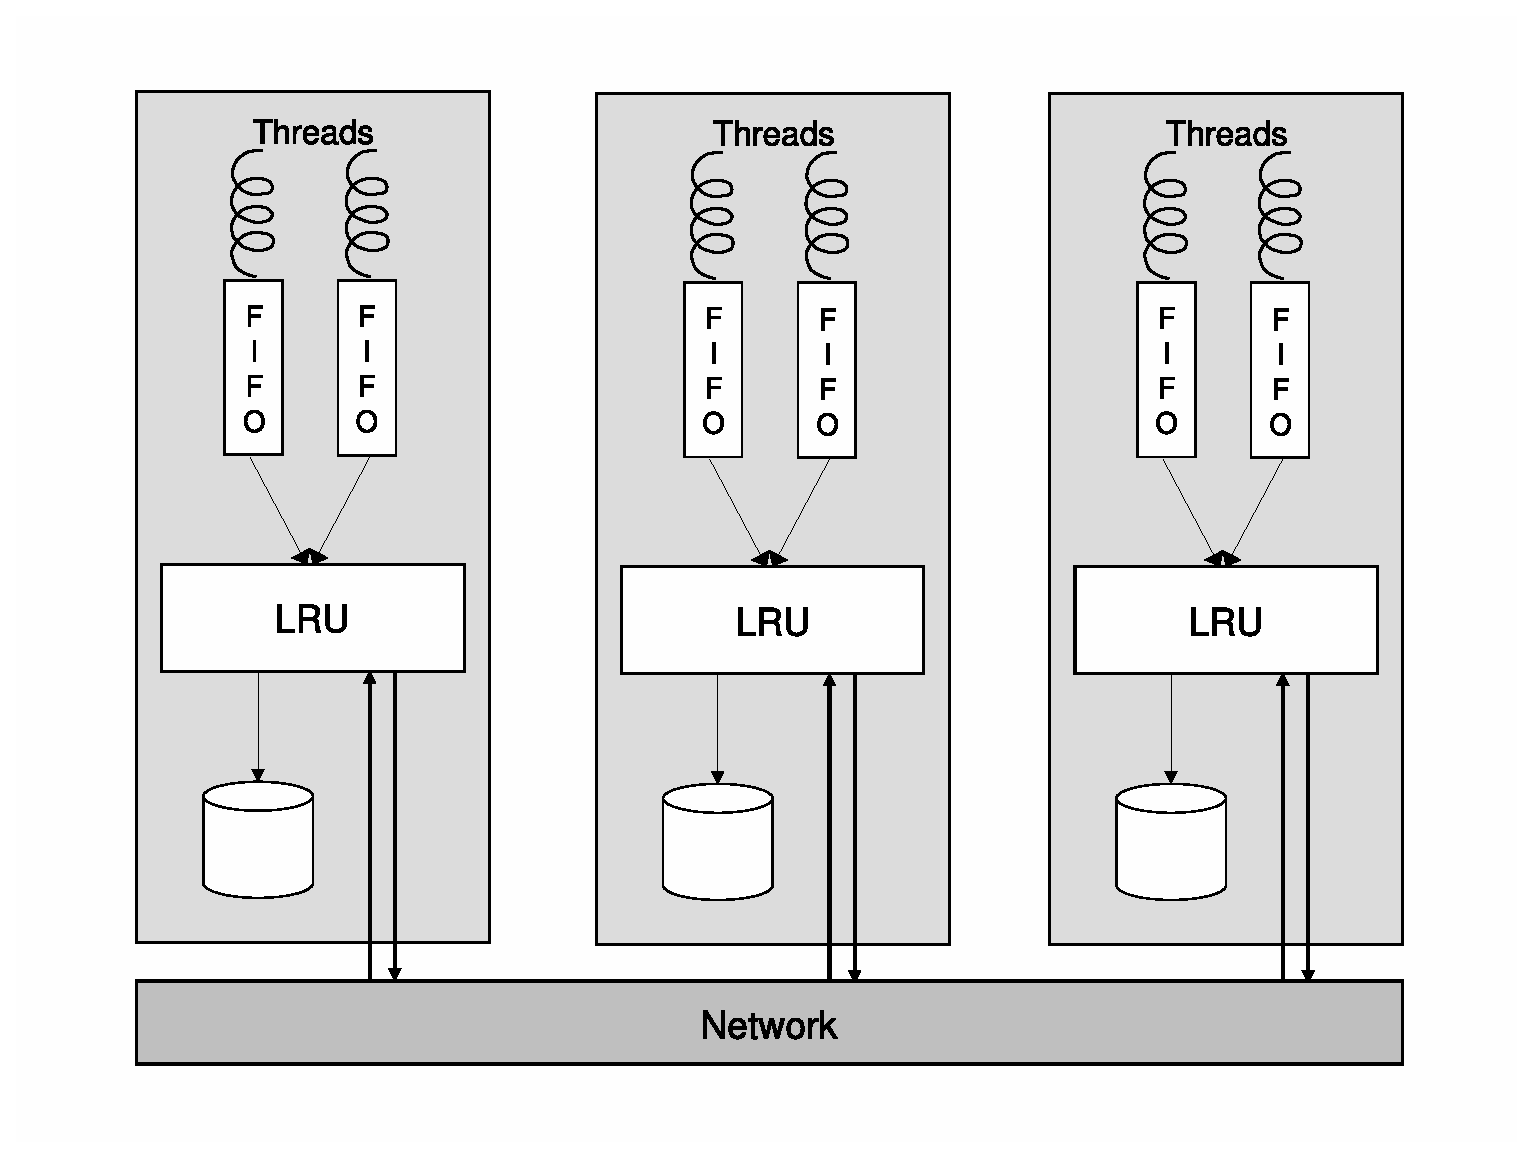
\includegraphics[width=3.5in,height=2.3in]{DistributedArchitecture.eps}
  \vspace{-.3in}
  \
  \caption{\label{fig:cache} A single distributed cache in THOR.}
\end{figure}

The primary cache is a set-associative LRU cache\footnote{We use 16-block sets, although we omit empirical evidence that a 4-way cache is nearly as good as a fully associative one.} that is shared among all threads.
Each cache maintains for each block which machine each it resides, whether it is in memory, and if out-of-core execution is permitted and it is local, its location on local disk.
Blocks are requested from its location and locked into memory on first use, and when unlocked, placed in the set-associative cache.
Unlike most distributed caches, we use a remarkably simple coherency protocol.
Simultaneous reads and writes to the same block are permitted if they are restricted to explicitly declared disjoint contiguous regions.
When the block is purged, only the overlapping contiguous regions are written.
Global consistency is ensured at global synchronization points, which occur after all computation has finished.

To avoid contention and caching overhead, each thread has a small (about 64 blocks) FIFO cache of blocks locked into memory.
The user code locks blocks into the FIFO cache\footnote{The FIFO's sizee places a hard limit on the number of active blocks.  Fortunately, 64 blocks is quite generous for balanced tree traversals.}.
Blocks are evicted to the set-associative cache in a round-robin fashion, skipping locked blocks.

{\bf Data layout.}
\THOR stores points are in tree-based skewed Morton ordering.
Additionally, we build the $kd$-tree such splits are aligned to block boundaries until a single block is reached, ensuring a one-to-one mapping between tree nodes and blocks of points.
Thus, storage spatial locality mirrors the metric spatial locality.
Tree nodes are stored pre-order, ensuring that subtrees correspond to contiguous ranges of nodes, and thus can be manipulated using our coherence model.

Nodes and points are then distributed block-by-block via the above domain decomposition.
If tree sections cross block boundaries, a tiebreaker is used.

\subsection{Scheduling}

... reread the banicescu paper
...

In earlier sections, we declared that a software system attempting to parallelize {\it any} generalized $N$-body problem cannot assume the ability to predict run times with the accuracy available via a dry run, when a dry run may take as much time as an actual computation.
Instead, we dynamically assign tasks to processors during the course of computation.
Each worker requests an item of work rom a central scheduler upon becoming idle.

The query tree is divided into a number of work items of roughly equal cardinality.
This is done quickly by choosing a minimum number of items $\hat{k}$, and performing a depth-first recursion until a subtree with at most $\frac{n}{\hat{k}}$ points is found.
We choose $\hat{k}$ to be a small constant factor times the total number of threads.

We then present two dynamic scheduling algorithms based on this model.
The first algorithm, which we call random-assignment, simply assigns a random task to a processor.
%If the tree is not balanced, it may also be beneficial to assign the largest-cardinality items first such that the smaller items can act as a buffer towards the end to increase balance.
The overhead of this scheduler is small -- $O(\hat{k})$ for the decomposition, and $O(\hat{k})$ for the work assignment.

Our second algorithm, which we call centroid tree-decomposition, attempts to manage communication cost by taking advantage of the fact that spatial locality mirrors data locality.
We start with an initial tree-based decomposition to assign preferred work items to machines, and provide a separate scheme to satisfy workers that have completed all initial tasks.

In a manner similar to the ORB dissection, we use the $kd$-tree itself starting at the root to assign each branch to a subset of machines, until we reach a single machine\authorsnote{Picture and-or pseudocode.  I promise that the algorithm is very simple.}.
We then further divide the subtree into pieces of cardinality at most $\frac{n}{\hat{k}}$, and assign all of these to the machine.
When a machine requests work, a task is assigned from this list if possible, but if it is exhausted, an overflow heuristic is used.
The goal of such a heuristic is to find a work item whose locally essential tree has the most data in common with previous work items, but also expected future work items.

One such heuristic is to find an unassigned work item closest to a centroid computed from the tasks a machine has already completed.
In severely nonuniform load, this centroid should gradually migrate to the new tasks that are assigned.
Optimally the set of work should have relatively low "surface area" compared to its "volume" -- a centroid that migrates too slowly opportunistically finds further and further "holes," but a centroid that migrates too quickly carves a finger-like path.
Our implmentation takes the mean of the midpoint of each task that has already been assigned to a machine.
Better heuristics may be possible, especially ones which take into account a more accurate model of correlation between locally essential trees for the particlar algorithm -- for instance, algorithms whose locally essential tree is almost exactly the same as the query tree would benefit only from extremely close work items, whereas the difference between somewhat or extremely distant work items is negligible.

The centroid scheduler has overhead $O(\hat{k})$ for tree decomposition, since it is also just a simple tree recursion.
To accelerate work assignment, which is worst-case $O(\hat{k}$ per assignment or $O(\hat{k}^2)$ total, we use a single-tree nearest-neighbor search.
However, since scheduling is such a small cost compared to the dual-tree computation, we are unable to measure this overhead.

%Our initial demonstrations use simple bag-of-tasks scheduling algorithm that adapts to problems where the execution time is bounded $a|Q| \leq t \leq aw|Q|$ where $a$ is the minimum ratio of query tree size to execution time, and $w$ is the maximum constant factor deviance from proportionality.

%In a bag-of-tasks system, each worker requests a new item of work from a central scheduler every time it becomes idle.
%Given identically sized subtrees of the query tree, the worst-case scenario is that $k - 1$ tasks taking time $t$ each are executed in perfect parallelism and terminate these at the same time, until the last task of length $wt$.
%The total time is then $\frac{(k-1)t}{p}+wt$, compared to the ideal run time $\frac{(k-1+w)t}{p}$.
%The utilization $u$ is then $\frac{k-1+w}{k-1+wp}$.
%For a minimum utilization of $u$, one needs at least $k = \frac{w+wpu}{1-u}+1$ tasks, asymptotically $\frac{wp}{1-u}$.
%For 50\% utilization with run times deviating from proportionality by a factor no more than 10, one needs a few more than $20p$ tasks.
%In practice, utilization is far better given this number of tasks.

%Extending the bag of tasks system, we attempt to minimize the amount of extra information a processor requires to take on its next work item.
%Since spatial locality mirrors data locality, we present a simple greedy algorithm.
%When a machine requests a work item, the next work item is the closest chunk of the query tree to the work items it has already performed.

%- haven't really implemented this, i'll get back as to the effectiveness

%- link spatial locality with data locality
%- phrase locality nicely
%The next query node that is assigned to a worker .

%So far, we have detailed in entirety the functionality of our multithreaded parallel software.

\section{Experimentation}

- What is the overhead of the caching architecture, and how many FIFO misses occur

- What is the overhead of task decomposition

- Multithreaded performance

- Cluster performance

\section{Future Work}

Future work mainly focuses on higher-quality and specialized implementations.
A future implementation may be aware of its cache and postpone tree traversals on parts of the tree that are not in cache.
Also, scalability to many more processors may be possible given specialized knowledge of the cluster, whether it is a datacenter environment with replicated distributed data, a large shared-memory system, or a multi-core\authorsnote{Elaborate some more.}.

Also, algorithms with more than two trees should parallelize in a manner similar to the existing ones.

%\nocite{ex1,ex2}
\bibliographystyle{abbrv}
\bibliography{paper}

\begin{appendix}

\section{Notation}

We're still working on our notation (in fact, all of the symbols we use are a user-defined command in LaTeX).

\begin{table*}
\begin{tabular}{|l|l|l|}
\hline
Symbol & Macro & Description, Rationale
\\ \hline $\kdroot{X}$ & kdroot & root node of spatial tree
\\ $\kdleft{X}$ & kdleft & left child of spatial tree node
\\ $\kdright{X}$ & kdright & right child of spatial tree node
\\ $\kdparent{X}$ & kdparent & parent of spatial tree node
\\ \hline $\Theta$ & Theta & a second-order reduce problem
\\ $\Gnp$ & Gnp & postprocessed second-order reduce problem
\\ $\gnp$ & gnp & second-order reduce problem computation before postprocess
\\ $\summary$ & summary & initial summary results
\\ \hline $\letterglob$ & letterglob & single-operator reduce 'problem space'
\\ $\outglob$ & outglob & single-operator reduce after postprocessing
\\ $\inglob$ & inglob & single-operator reduce before postprocessing
\\ $\Opglob$ & Opglob & single-operator reduce operator
\\ $\fglob$ & fglob & single-operator reduce inner function
\\ $\gglob$ & gglob & single-operator reduce postprocess
\\ $\canpruneglob$ & canpruneglob & single-operator reduce prune function
\\ $\deltaglob$ & deltaglob & single-operator reduce prune value
\\ \hline $\letterqr$ & letterqr & query-reference 'problem space'
\\ $\outqr$ & outqr & query-reference after postprocessing
\\ $\inqr$ & inqr & query-reference before postprocessing
\\ $\Opqr$ & Opqr & query-reference operator
\\ $\fqr$ & fqr & query-reference inner function
\\ $\gqr$ & gqr & query-reference postprocess
\\ $\identqr$ & identqr & identity element of abelian monoid $\Opqr$
\\ $\letterqrv$ & letterqrv & mass result 'problem space'
\\ $\inqrv$ & inqrv & mass result function
\\ $\deltaqrv$ & deltaqrv & mass result prune value
\\ $\canpruneqrv$ & canpruneqrv & query-reference prune check
\\ $\varqrv$ & varqrv & accumulator to build up $\inqrv$
\\ $\varqrvparent$ & varqrvparent & 'parent' values of $\inqrv$ from upwards prunes
\\ \hline $\lettermu$ & lettermu & query-reference summary values
\\ && 'problem space'
\\ $\inmu$ & inmu & summary result function
\\ $\Outopmu$ & Outopmu & summary result query-summarization
\\ $\Opmu$ & Opmu & summary result reference-joining
\\ $\fmu$ & fmu & inner function converting $\inqr$ to $\inmu$
\\ $\fmuv$ & fmuv & inner function converting $\inqrv$ to $\inmu$
\\ $\deltamu$ & deltamu & 'initial' summary results
\\ $\canprunemu$ & canprunemu & prune check for extrinsic prunes
\\ $\identmu$ & identmu & identity element of abelian monoid $\Opmu$
\\ $\heurqr$ & heurqr & expansion heuristic
\\ $\varmuchild$ & varmuchild & high-quality, built bottom-up with $\Outopmu$
\\ $\varmuparent$ & varmuparent & low-quality, built top-down with $\Opmu$
\\ \hline $\letterstat$ & letterstat & statistic 'problem space'
\\ $\outstat$ & outstat & statistic after postprocessing
\\ $\instat$ & instat & statistic before postprocessing
\\ $\Opstat$ & Opstat & combining statistics
\\ $\fstat$ & fstat & statistic inner function
\\ $\gstat$ & gstat & statistic postprocessing function
\\ \hline
\end{tabular}
\caption{Notation used throughout the paper.}
\label{tab:notation}
\end{table*}

\end{appendix}

\end{document}

